\scanpage{112}
% archive foliation: 111
Donc on voit que les zéros de $P(c)$ sont distincts de $0,1$ et ne sont pas des zéros de $Q$. Mais pourraient-ils être zéros de
\[
\delta(c)=25c^2-32c+16\quad ?
\]
\figure{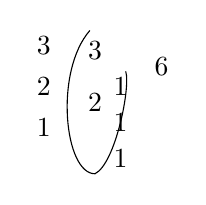
\begin{tikzpicture}[scale=.65]
\node at (0,2){$3$};\node at (0,1.2){$2$};\node at (0,.4){$1$};
\node at (1,1.9){$3$};\node at (1,.9){$\deleted{\unsure{2}}$};
\node at (1.5,1.2){$1$};\node at (1.5,.5){$1$};\node at (1.5,-.2){$1$};
\draw (.9,2.3)..controls(.2,1.5)and(.4,-.5)..(1,-.5)..controls(1.4,-.3)and(1.7,1.2)..(1.6,1.5);
\node at (2.3,1.6){$6$};\end{tikzpicture}}
\[
f'(z)=0\Rightarrow f(z)=0
\]
\deleted{\figure{\begin{tikzpicture}[scale=.6]
\node at(-.8,1){\unsure{ou}};\node at(0,1){$3$};\node at(0,.4){$2$};\node at(0,-.3){$1$};\draw(0,.35)ellipse(.4 and1);
\node at(1.4,.7){$\unsure{0}$};\node at(3.4,1){$3$};\node at(3.4,.1){$1_3$};\draw(3.4,.5)ellipse(.25 and.9);
\draw(-.7,.7)..controls(1,1.8)and(.4,-.5)..(1.5,.6)..controls(2.4,1)and(1.5,-.1)..(3.8,.8);
\end{tikzpicture}}}
\[
f(z)=\lambda\frac{\varphi}{\psi}
\]
\margin{$\varphi,\psi$ \inserted{unitaires} premiers entre eux à zéros indéterminés de multiplicités données, $\deg\varphi>\deg\psi$}
\[
\frac{f'(z)}{\inserted{f(z)}}=
\deleted{\frac\lambda{\psi^2}}
\left(\frac{\varphi'}{\inserted{\varphi}}\deleted{\psi}
-\frac{\psi'}{\inserted{\psi}}\deleted{\varphi}\right)
\]
\[
\sum\frac{p_i}{z-\alpha_i}\ \unsure{*}\ \unsure{-}\sum\frac{\unsure{5|q_j}}{\unsure{z}-\beta_j}
\]
\[
=\frac1{\prod(z-\alpha_i)\prod(z-\beta_j)}\;\bigl(\qquad\bigr)
\]
